\namedsection{Programmiersprachen}{J}
Allein der Vergleich zwischen zwei Programmiersprachen könnte vermutlich einen ganzen Bericht füllen. Gerade deshalb sollte es klar umrissene Kriterien geben die bei der Gewichtung helfen. Diese werden bereits zu beginn ausführlich diskutiert.
Im nächsten Abschnitt werden mehrere Programmiersprachen auf Grundlage unserer zuvor diskutierten Kriterien verglichen und eingeordnet.
Zuguterletzt werden die Ergebnisse der Evaluierung tabellarisch zusammengefasst und kritisch hinterfragt.

\subsection{Evaluierungskriterien}
Für jedes Kriterium werden wir kurz beschreiben was es bedeutet und anschließend ausführen warum es für unser Projekt von Bedeutung ist.
\begin{description}
    \item [Performanz]
    Wie schlägt sich die Programmiersprache hinsichtlich Speicherverbrauch, CPU-Auslastung und Request-Durchsatz?
    Wenn die Sprache einen geringeren Speicherverbrauch aufweist, kann die Chunk-Größe für die Batchjobs vergrößert und dadurch die Zeit bis zur Abarbeitung verkürzt werden.
    Wenn der Request-Durchsatz hoch ist, können mehr Anfragen pro Zeiteinheit bewältigt werden was der Skalierbarkeit zugute kommt.
    \item [Verbosität]
    Wie effizient ist die Sprache hinsichtlich ihrer Syntax? Lässt sich mit wenig Code bereits viel bewältigen? Wie schnell lassen sich mit der Sprache Resultate erzielen?
    Wenn es sich mit einer Sprache besonders produktiv arbeiten lässt können bessere Resultate in gleicher Zeit erzielen.
    \item [Ökosystem]
    Wie groß ist die Community? Wie gut lassen sich weitere Bibliotheken und Dokumentationen finden?
    Umso mehr Informationen frei zur Verfügung stehen desto schneller kann man eventuelle Probleme aus dem Weg räumen oder sich in Sprachkonzepte einarbeiten (z.B. Multithreading).
    \item [Erfahrungen]
    Wie viel Vorwissen besitzen die Teammitglieder mit der Programmiersprache?
    Bereits vorhandenes Wissen nutzen um effizienter zu einer Lösung kommen zu können.
    \item [Sonstiges]
    Was sind weitere erwähnenswerte Eigenschaften der Sprache oder Bestandteile des Ökosystems?
    Es könnte bereits Clients für Drittsysteme geben oder einige Eigenschaften der Sprachen kommen unserer Architektur besonders entgegen.
\end{description}

\subsection{Betrachtete Programmiersprachen}
Die Wahl der untersuchten Programmiersprachen hängt auch mit der Wahl der untersuchten Frameworks zusammen. Insofern werden in diesem Abschnitt die Programmiersprachen Java, C\#, JavaScript (und TypeScript), PHP sowie Python betrachtet.

Um die Informationen aus den Tabellen \ref{tab:comp_pl1} und \ref{tab:comp_pl2} besser einordnen zu können folgt eine kurze Erläuterung zu den wichtigsten Spalten und Quellen. In vielen Fällen ergeben sich die endgültigen Ergebnisse aus der Aggregation aller Daten der Quellen.

Mit Request-Durchsatz ist in der Regel die Anzahl der bearbeiteten Anfragen pro Zeiteinheit bei gleichwertiger Hardware gemeint. In den aufgeführten Quellen wurde dies auf unterschiedliche Weise probiert. Entweder mit Server die direkt ohne weitere Operation antworten oder die Aufgaben mit typischen Arbeiten im Lebenszyklus eines Servers emulieren.

Die CPU-Performanz bezieht sich auf die Laufzeit und Auslastung von Arbeitseinheiten für unterschiedliche Programmiersprachen. Eine Programmiersprache die effizienter arbeitet indem sie die Aufgabe in kürzerer Zeit abarbeitet oder CPU-Kerne besser auslastet wird demzufolge besser bewertet. Für diesen Punkt wurde vornehmlich das Benchmarks Game betrachtet und alle Werte verglichen.

Die Spalte mit der Bezeichnung "Umfang Third-Party" enthält gesicherte Angaben über die Anzahl einzigartiger Bibliotheken aus den meistgenutzten Third-Party-Datenbanken der jeweiligen Programmiersprache. Erwähnenswert ist in diesem Zusammenhang, dass man die Werte für npm kritisch betrachten sollte, weil JavaScript insbesondere im Frontend-Umfeld genutzt wird. Dadurch hat JavaScript im Vergleich zu anderen auch viel mehr grafische Komponenten als Bibliotheken. Darüber hinaus gibt es keine zuverlässige Auskunft über die Qualität einzelner Bibliotheken in den jeweiligen Third-Party-Datenbanken.

Der Punkt Community wertet vor allem diverse Ranglisten zur Popularität der Sprachen aus. Unser Ansatz ist die Überlegung, dass eine höhere Popularität auch mit mehr hilfreiche Quellen für die Programmiersprachen einhergehen. In der Regel greifen diese Ranglisten in vielen Fällen auf Informationen wie Anzahl der Ergebnissen aus Suchmaschinen zurück. Für präzisere Informationen wurde auch auf Daten von Stackoverflow und Github zurückgegriffen.

\begin{table}[H]
    \centering
    \begin{tabular}{|p{3cm}|p{5cm}|p{5cm}|}
    \hline
    \textbf{Programmier- sprache}          & \textbf{C\#}                                                                & \textbf{Java}                                                           \\ \hline\hline
    Erschienen                     & 2000                                                               & 1995                                                           \\ \hline
    Programmier- paradigma \cite{wiki_pl}           & vornehmlich objekt-orientiert mit Ausätze für andere Paradigma     & vornehmlich objekt-orientiert mit Ausätze für andere Paradigma \\ \hline
    Statisch / Dynamisch typisiert \cite{wiki_type} & statisch                                                           & statisch                                                       \\ \hline
    Stark / Schwach typisiert \cite{wiki_type}      & stark                                                              & stark                                                          \\ \hline
    Intepretiert                   & ja (Bytcode)                                                       & ja (Bytecode)                                                  \\ \hline
    Speicherverwalt- ung             & Garbage Collector                                                  & Garbage Collector                                              \\ \hline
    Multithreading                 & ja                                                                 & ja                                                             \\ \hline
    Request-Durchsatz \cite{mihai_benchmark,tandemseven_perf,techempower_benchmark,benchmark_web,medium_awslambda,acloud_awslambda}              & gut                                                                & sehr gut                                                       \\ \hline
    CPU-Performanz \cite{benchmark_game,benchmark_kostya}                & sehr gut                                                           & sehr gut                                                       \\ \hline
    Verwendung                     & Enterprise                                                         & Enterprise                                                     \\ \hline
    Erfahrungen                    & wenig                                                              & gut                                                            \\ \hline
    Umfang Third-Party             &  nuget ca. 180k \cite{csharp_packages}                           & gradle/maven ca. 315k \cite{java_packages}         \\ \hline
    Community \cite{stackoverflow_survey,tiobe,pypl,github_octoverse,redmonk}                      & moderat                                                            & sehr gut                                                       \\ \hline
    Anmerkungen                    & Third-Party Bibliotheken häufig kommerziell ausgelegt, Typsystem & OFTP Client/Server Referenzimplmentierung verfügbar, Typsystem \\ \hline
    \end{tabular}
    \caption {Vergleich Programmiersprachen C\# und Java}
    \label{tab:comp_pl1}
\end{table}

\begin{table}[H]
    \centering
    \begin{tabular}{|p{3cm}|p{3.7cm}|p{3.7cm}|p{3.7cm}|}
    \hline
    \textbf{Programmier-sprache}                                                                        & \textbf{JavaScript (Node.js)}                                                              & \textbf{Python}                                                  & \textbf{PHP}                                                                                                \\ \hline\hline
    Erschienen                                                                                   & 1995 (2009)                                                                        & 1990                                                    & 1995                                                                                               \\ \hline
    Programmier- paradigma \cite{wiki_pl} & ursprünglich prozedural, mittlerweile Ausätze für andere Paradigma, keine Generics & vornehmlich prozedural mit Ausätze für andere Paradigma & vornehmlich objekt-orientiert mit Ausätze für andere Paradigma, keine Generics, nicht event-driven \\ \hline
    Statisch / Dynamisch typisiert \cite{wiki_type}                                                              & dynamisch                                                                          & dynamisch                                               & dynamisch                                                                                          \\ \hline
    Stark / Schwach typisiert \cite{wiki_type}                                                                   & schwach                                                                            & stark                                                   & schwach                                                                                            \\ \hline
    Intepretiert                                                                                 & ja                                                                                 & ja                                                      & ja                                                                                                 \\ \hline
    Speicherverwalt -ung                                                                        & Garbage Collector                                                                  & Garbage Collector                                       & Garbage Collector                                                                                  \\ \hline
    Multithreading                                                                               & ja                                                                                 & ja                                                      & ja                                                                                                 \\ \hline
    Request-Durchsatz \cite{mihai_benchmark,tandemseven_perf,techempower_benchmark,benchmark_web,medium_awslambda,acloud_awslambda}                                                                           & I/O intensiv sehr gut \cite{performance_io}                                                              & moderat                                                 & gut                                                                                                \\ \hline
    CPU-Performanz \cite{benchmark_game,benchmark_kostya}                                                                               & gut                                                                                & moderat                                                 & moderat                                                                                            \\ \hline
    Verwendung                                                                        & Frontend, API                                                                      & Datenanalyse, Machinelles Lernen, Automatisierung     & Web Backend, API                                                                                   \\ \hline
    Erfahrungen                                                                                  & gut                                                                                & wenig                                                   & wenig                                                                                              \\ \hline
    Umfang Third-Party                                                                           & npm über 1 Million \cite{js_packages}                                    & pip pypi ca. 210k \cite{python_packages}              & composer packagist ca. 250k \cite{php_packages}                                \\ \hline
    Community \cite{stackoverflow_survey,tiobe,pypl,github_octoverse,redmonk}                                                                                    & sehr gut                                                                           & sehr gut                                                & gut                                                                                                \\ \hline
    Anmerkungen                                                                                  & JSON ist Bestandteil der Sprache                                                 & ~                                                       & ~                                                                                                  \\ \hline
    \end{tabular}
    \caption {Vergleich Programmiersprachen JavaScript, Python und PHP}
    \label{tab:comp_pl2}
\end{table}

Nun zurück zur eigentlichen Gegenüberstellung. Grundsätzlich haben Java und C\# aufgrund ihrer Beschaffenheit hinsichtlich dem vorherigen kompilieren zum Bytecode und dem Ansatz bzgl. der dynamischen und starken Typisierung einen Performance-Vorteil. Dieser spiegelt sich, wie bereits zuvor erwähnt, auch in einigen Benchmarks wieder. Jedoch fehlt für C\# den meisten Teammitgliedern an Erfahrung und auch das Ökosystem ist im Vergleich zu Java bedeutend kleiner, sodass auch das einarbeiten aufwändiger wäre.

Demgegenüber könnte man Java und JavaScript (bzw. TypeScript) stellen, welche ein ähnlich starkes Ökosystem bieten und bei denen auch die Vorerfahrungen im Team ähnlich sind. Allerdings kann JavaScript längst nicht so stark in Punkto Typesicherheit, Multithreading und CPU-Effizienz auftrumpfen. Zusätzlich bietet Java den Vorteil, dass es z.B. für QDX eine Referenzimplementierung gibt.

Man könnte vielleicht noch argumentieren, dass Python im Bezug auf Verbosität einen Vorteil für die Produktivität haben könnte \cite{expressiveness}. Dem kann man gegenüberstellen, dass durch Frameworks wie Spring Boot und Bibliotheken wie Project Lombok die Verbosität bei Java geradezu minimal ist. Mehr Informationen darüber gibt es im Abschnitt \ref{sec:libraries}.

\subsection{Auswertung und Diskussion}

Insgesamt lässt sich also zusammenfassen, dass Java für uns die beste Wahl ist. In der Tabelle \ref{tab:programming_language_evaluation} können nochmal die einzelnen Kriterien und Bewertungen auf einer Skala von 1 - 5 für jede Programmiersprache eingesehen werden.
\begin{table}[!h]
\centering
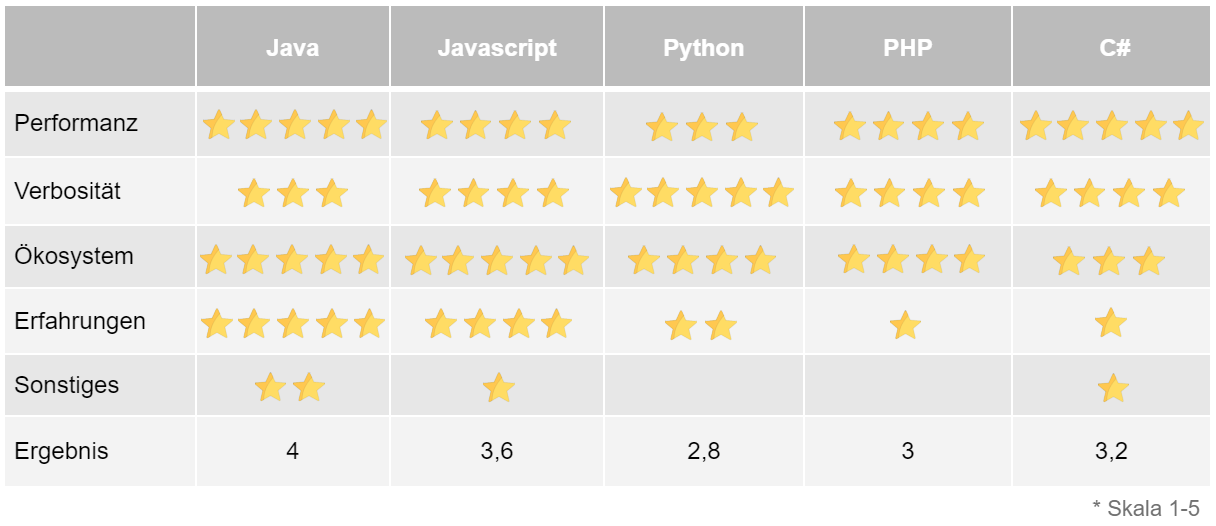
\includegraphics[width=14cm]{images/0x_technology_stack/programming_language_comparison_table.png}
\caption{Auswertung Programmiersprachen.}
\label{tab:programming_language_evaluation}
\small{Sonstiges sind Bonus-Punkte}
\end{table}

Generell hilft es für das Verständnis der Analyse für Programmiersprachen unsere Auswertung im Kontext unserer Architekturwahl zu sehen. Mithin hängt sie inhaltlich auch stark mit der Analyse für die Frameworks zusammen. Viele der hier aufgeführten Ergebnisse werden vermehrt auch in den Abschnitten zu den Frameworks genutzt.

Gerade im Umfeld von Datenintegration ist davon auszugehen das Reserven bei Speicher-Auslastung und die höhere CPU-Effizienz bei Java einen wichtigen Vorteil gegenüber den meisten anderen Sprachen haben.

Ebenfalls nicht unerwähnt bleiben sollte der Umstand bei JavaScript, dass theoretisch auch als Grundlage für die Entwicklung anstatt Node.js auch $\mu$WebSockets (wird unter anderem für Crypto-Handelsplatz Coinbase genutzt) gewählt werden könnte, dass mit einer immensen Performancesteigerung bei den Request-Durchsatz einhergeht. Mit dem Nachteil, dass viele Bibliotheken aus dem JavaScript Ökosystem nicht mehr ohne weiteres genutzt werden können.
